\section*{Design}

Delivering messages, critical and casual, to mobile users and
endpoints that are interested in them is the overarching premise of
this work. Our vision for realizing an end-to-end mobile message
delivery service design principles revolve around {\bf X} central
goals:

\begin{itemize}
\item Relevant content

The service should provide mechanisms to target groups of endpoints
which have explicit or implied interest in messages. A message may be
important because an end user specifically asked for the content based
on its attributes (nearby gas prices). Alternatively, a message may be
deemed relevant for the endpoint because it is related to an emergent
event (vehicle accident ahead).

\item Robust, low overhead, low latency communication

Message intent drives content delivery requirements.  For example,
different types of emergency service messages have been identified for
VANETs, each having distinct latency
requirements~\cite{vanet-msg-reqs}. The service should strive to
minimize latency to provide on-time delivery with headroom for outlier
delays. Messages should be categoriezed according to their relative
importance and processed accordingly (e.g., emergency info before
consumer content).

\item Flexible deployment

Adoption of the service is bolstered by adaptability to different
mobile networking environments.  Such accomodation allows for
deployment into LTE networks with different geographic EPC service
placements and degrees of maleability.  The service should allow for
centralized metropolitan area integration (CloudRAN) and distributed
edge deployment (peer-to-peer eNodeB).

\item Message trust and integrity

Messaging is vulnerable to various attacks, particularly if peers are
used as transits such as in 802.11p multihop clusters. A combination
of PKI, message integrity checks, and centralized vetting should be
employed to curtail abuse and instill trust.

\item Reuse of effective technologies

It is our contention that an end-to-end service should not supplant
existing mechanisms useful for achieveing its composition.  Indeed, it
is counterproductive to introduce new service components that induce
unnecessary changes and capital investments. The messaging service
should strive to work alongside existing mobile network protocols and
services.  Only where existing mechanisms do not provide key
functionality or do not give adequate service levels should changes be
introduced.  Such changes should be as minimal and transparent as
possible to foster compatibility and ease of adoption. On the other
hand, considering less constrained future mobile network
architectures~\cite{5G}~\cite{venkataramani2014mobility} is also important.

\end{itemize}

We next describe the components of the Mercury messaging system, along
with how they fit into the 3GPP 4G mobile networking architecture.

%%% ARCHITECTURE FIGURE
\begin{figure}[h]
  \begin{center}
    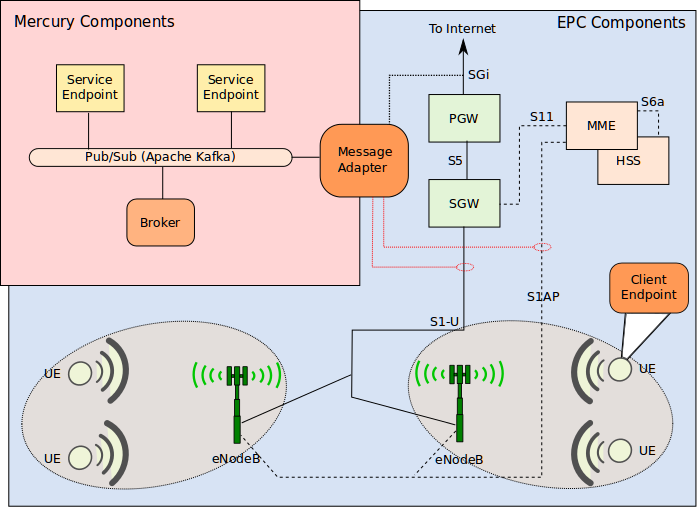
\includegraphics[width=0.5\textwidth]{figs/mercury-arch.png}
    \caption{Mercury architecture diagram (in 4G mobile network context)}
    \label{fig:arch}
  \end{center}
\end{figure}

\subsection{Mercury Components}

Mercury is comprised of four essential components: message broker,
publish/subscribe system, message adapter, and endpoint.  These
components are visible in the architecture diagram in
figure~\ref{fig:merc-arch}. This diagram shows the Mercury components
in the context of a 4G mobile network (the latter will be described
after Mercury is covered).

\begin{itemize}

\item Publish/Subscribe System

Mercury makes use of the \pubsub pubsub system. Much work has been
done on pubsub systems, and it is not the aim of this work to provide
novel pubsub mechanisms. \pubsub provides ... {\bf discuss desirable
  attributes, such as scaling, performance, community support, and
  rich subscription capabilities, and how they are relevant}.

{\bf Discuss how Mercury integrates with the pubsub.}

\item Message Broker

Mercury's message broker is the brain center of the messaging
system. It processes all incoming messages and sends these to relevant
endpoints (via \pubsub). It also coordinates messaging system sessions
with the endpoints. The broker calculates Areas of Interest (see
section~\ref{section:aoi}) for certain message types (e.g., emergency
notifications).  Messages are vetted by the broker to prevent
spoofing, enforce authorized use, cull abuses (flooding, other DoS),
and perform system data analysis (endpoint reputation, problems with
coverage, etc.).

The broker forwards vetted and scoped messages to the pubsub system
for transmission to appropriate endpoints.  The broker does not
concern itself with how to get the messages to the target endpoint(s);
that job falls to the Mercury message adapter.

The message broker is horizontally scalable in a data center
environment. The implementation section discusses how a centralized
database and distributed in-memory caching is used to accomplish this.

\item Message Adapter

The Mercury message adapter is the conduit through which pubsub
messages flow through to endpoints. The prototype implementation
described in this paper targets the 4G EPC, but it is possible to
target other mobile networking architectures with different adapters.

The message adapter receives group membership updates from the
broker. This allows it to map (groups of) endpoints to destinations
within the mobile network.  For example, an adapter's domain may span
from a single eNodeB to multiple eNodeBs.  The message adapter
forwards messages toward endpoints (UEs) based where they are attached
and what state they are in.

\item Endpoints

Mercury endpoints are the producers and consumers of most content in
the messaging system. Many are client applications running on
ITS-equipped vehicles.  Such endpoints report in with telemetry, such
as their current position and speed.  Such endpoints also subscribe to
particular consumer messages identified by specified attributes.

Endpoints may also be centralized services that connect to the pubsub,
running at the same location (e.g., CloudRAN datacenter). Examples
include emergency notification processors, and consumer information
aggregators (gas prices).

\end{itemize}

\subsection{Mercury Messages}

Messages are the principle and only communication mechanism in
Mercury. There are two high-level flavors: control and
content. Control messages include session handling (between broker and
endpoints), broker to message adapter communication, and subscription
management (endpoint to pubsub/broker).  Content messages are those
relevant to applications running on endpoints, such as emergency
alerts and consumer information (e.g. gas prices).  Periodic session
maintenance messages are sent from mobile endpoints toward the broker
to update location and status.  The broker likewise sends periodic
heartbeat messages toward all endpoints. These messages ensure clients
and broker stay in sync. Session handling also includes establishment
and teardown message exchange.  Content messages use structured
message attributes to signal category information. This allows content
producer and consumer endpoints to steer messages to one another based
on interests. All messages flow through both the pubsub system and the
broker. The broker is always in the loop so that it can enforce sender
and message authenticity, perform flow control (rate limiting, etc.),
and compute metrics.

Messages have temporal and spatial relevancy.  Each message type,
including content messages, are valid within a bounded time
window. Further, certain message types have strict delivery deadlines
(emergency messages, inter-vehicle coordination). Such time bounds
necessarily restrict how Mercury can be deployed, as we discuss in
subsection~\ref{sec:deployments} below.

Message destination addressing in Mercury includes endpoint, content,
and area of interest targetting. Endpoint addresses are primarily used
for session setup and teardown. Content-specific addressing makes use
of subscription attributes to deliver messages. AOI addresses are
unique to the mobile environment. AOI bounds are computed by the
broker. These bounds form the destination address. Message adapters
check bounds to determine if their downstream area coverage is
relevant before passing along, and endpoints check their position
relative to the bounds.  In this way, Mercury allows messages to be
``area multicasted.''  Mercury's design vision includes using spatial
analysis techniques~\cite{sp-an1}~\cite{sp-an2} to create and test
bounds.  As we discuss in the implementation section, the prototype
restricts itself to simple bounding models (e.g., radius or current
route). Complex spatial reasoning for improving relevancy is left for
future work.

\subsection{Mobile Networking Ecosystem}

Mercury is primarily framed in the context of the 3GPP 4G and emerging
5G mobile networking architectures. Therefore, we provide some
background on these systems.  The vast majority of mobile carriers
utilize these Evolved Packet Systems (EPS)~\cite{mobile-stats}, making
them an especially relevant environment in which to operate a mobile
messaging system.  Note that Mercury is also amenable to other
mobility-friendly network architectures, such as
MobilityFirst~\cite{mobility-first}, but we focus the discussion in
this paper on the 3GPP EPS.  The 4G system has been in active
deployment for {\bf XXX} years, and has undergone a number of
revisions. We leverage features up through revision 12 of the 4G EPC
standards.  Also in play in some deployment scenarios (see
section~\ref{deployments}) are software defined infrastructure
concepts that are expected to be prominent components in the upcoming
5G EPS~\ref{5G-SDI}.

The 4G EPS includes the following key service functions relevant to
Mercury: Mobility Managment Entity (MME), Home Subscriber Service
(HSS), Serving Gateway (SGW), Packet Data Network Gateway (PDN-GW or
more commonly PGW), evolved NodeB (eNodeB), and User Equipment (UE).
We will briefly describe the role of each of these components, and
their relationships with one another and with Mercury. The Mercury
architecture diagram in figure~\ref{fig:merc-arch} shows Mercury
components in the context of a 4G EPS.  There are additional 4G
functions in this figure that we will cover in more depth when
discussing Mercury's design details.

\begin{itemize}

\item User Equipment (UE)

User Equipment typically refers to end user devices such as mobile
phones, tablets, and 4G radio equipped laptops.  The class of UE
devices also includes fixed-position equipment, such as alarm
controllers, remote telemetry systems, and other upcoming 5G Internet
of Things (IoT) devices. Particularly relevant to Mercury, UE devices
also include ITS endpoints (vehicles and road network infrastructure).

\item Mobility Management Entity (MME)

The MME is the 4G EPS control plane function responsible for tracking
the live (dynamic) session state for UEs. It manages session
setup/release, location tracking, handover between eNodeBs, and other
tasks. It coordinates interaction between UEs, eNodeBs, SGWs, and the
HSS. UE authentication and authorization are handled by the MME. In
some deployment scenarios, Mercury observes the MME signalling (S1-AP
protocol) to track device status and association.  Mercury also uses
the MME to setup and manage eMBMS bearers for multicasting messages to
endpoints.

\item Home Subscriber Service (HSS)

The HSS is essentially a database of user (subscriber) information.
The MME obtains UE information from the HSS based on mobile network
identifiers (typically the IMSI in 4G EPS). Authentication parameters,
QoS service levels, phone system parameters, and other information are
stored for UEs in the HSS.  Mercury does not make direct use of the
HSS, but we mention it because it is a key component of the EPC.

\item Serving Gateway (SGW)

The SGW is one of the two anchor points for connected UEs (the other
being the PGW). The SGW maintains GTP tunnels (which carry UE network
traffic) between itself and the downstream eNodeB, and also an
upstream PGW. Handovers between eNodeBs within a particular area
typically involve migrating the same SGW's downstream tunnel between
the two.  Handover can be seamlessly handled such that it is largely
invisible to the UE; its IP address stays the same, and its
connections remain open.  The upstream GTP tunnel to the PGW stays in
place across handovers.  In some deployments, Mercury taps into the UE
data tunnel between eNodeBs and the SGW to extract messages at a
location closer to the edge (e.g., in a CloudRAN data center).

\item Packet Data Network Gateway (PDN-GW, or PGW)

PGWs are frequently deployed in centralized datacenters in mobile
carrier networks.  They act as the egress point for a large number of
UE data bearers (GTP tunnels), and fan out to multiple SGWs. PGWs
forward UE trafic along toward a target network, which is frequently
the Internet, but may be a corporate network or IMS (for VoLTE
calls). PGWs enforce QoS, usually based on the subscriber's plan with
the carrier. They also do traffic accounting, reporting to billing and
charging functions. As with the HSS, Mercury does not make direct use
of the PGW. In some deployments, Mercury sends and receives endpoint
messages immediately upstream of the PGW device.

\item Evolved NodeB (eNodeB)

eNodeBs are the wireless access points of the 4G EPS. They bridge the
radio access network (RAN) through which the UEs directly communicate
with the evolved packet core (EPC). GTP tunnels are established for
each UE device between the eNodeB it is associated with and an
upstream SGW.  The eNodeB also initiates session setup and default
data bearer establishment when UE devices attach. It acts as a proxy
for UE to MME control plane signalling (Non-Access Stratum (NAS) over
S1-AP). eNodeBs covering adjacent cells coordinate through the MME and
possibly with one another to accomplish handover as UEs move. In the
distributed peer-to-peer deployment scenario, Mercury components run
directly on the eNodeBs.

\end{itemize}

\subsection{Deployment Scenarios}

%%% DEPLOYMENT SCENARIOS DIAGRAM.
\begin{figure}[ht]
  \begin{center}
    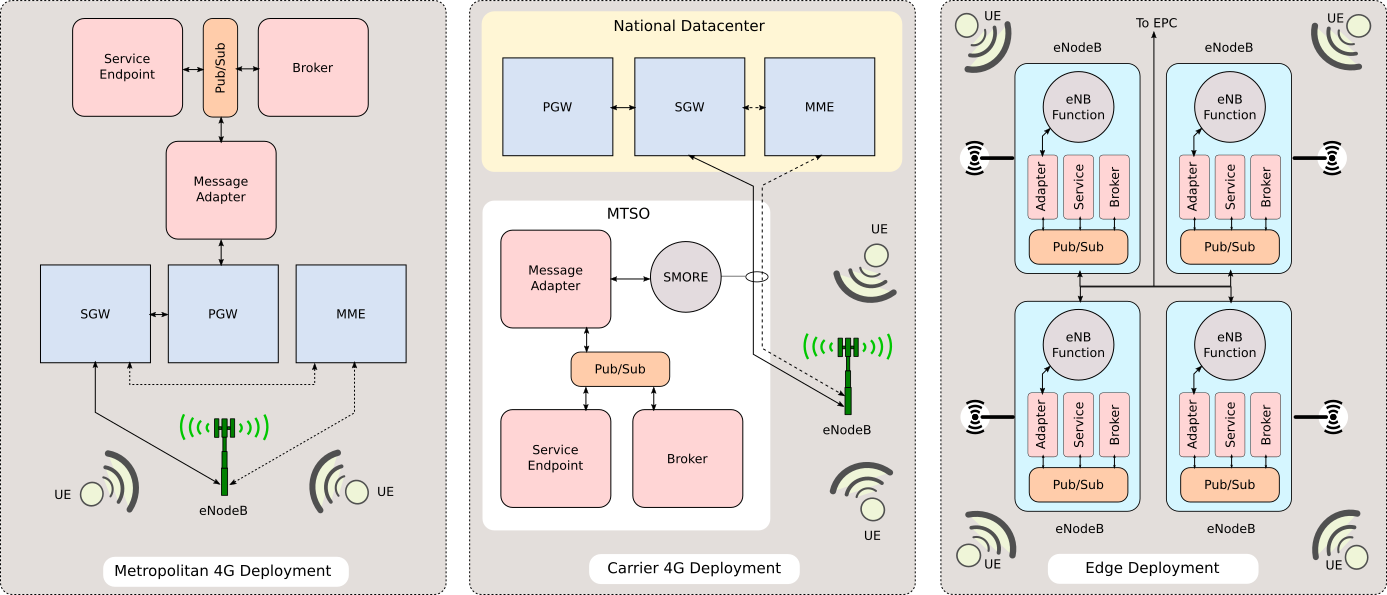
\includegraphics[width=0.5\textwidth]{figs/deploy.png}
    \caption{Mercury deployment scenarios.}
    \label{fig:deployments}
  \end{center}
\end{figure}

A key aspect of the Mercury design is adaptability to different mobile
network deployments and architectures. Endpoints, broker, and pubsub
components are all mobile-environment agnostic. Mobile endpoint
identity is specific to the Mercury messaging system. The message
adapter's primary function is to separate the concerns of the
messaging system with the routing of messages inside the mobile
network.  Mercury requires a low-latency vantage point near the mobile
network edge. Message adapters, pubsub, and broker all need to reside
at this vantage point.  Such proximity allows for message delivery to
meet timing SLAs.  Distance to endpoints incurs a tradeoff between
convenience of deployment and ability to meet timing needs. We show
deployment versus distance/latency requirements in
table~\ref{tab:lat-req}.

{\bf ADD DEPLOYMENT VS. LATENCY TABLE}

The message adapter can utilize different techniques to interface with
a mobile network deployment. In the simplest case, it can interact
with endpoints via routed network addresses (e.g. IPv4 or
IPv6). Alternatively, it may transparently interpose on encapsulated
communication channels to inject/extract messages (e.g. GTP
bearers). Another option is for the message adapter to operate in
concert with the wireless access point right at the edge. It could do
this by transparently interposing on the access point's data plane
uplink, or via an integrated side channel added into the access point
software.  We present next three plausible deployment scenarios.

\begin{itemize}

\item Metropolitan area 4G deployment

Consider a city investing in Intelligent Transportation System
infrastructure. Resources include a data center within the city and
wireless coverage via eNodeBs (particularly along major vehicle
corridors). The 4G EPC components reside in the local data center,
including the PGW.  Given a maximum cabling distance from the data
center to any eNodeB of around 100~kilometers, one way speed of light
latency is bounded to less than 5~milliseconds.  LTE one-way wireless
first-hop target latency is 5~ms, but may be more like
10~ms~\cite{RAN-latency} due to UE and eNodeB processing overhead.
Further switch/router hops within the data center should not
appreciably add to the latency. Egress through SGW/PGW can add another
5~ms of one-way delay~\cite{EPC-latency}.  Total mobile network
infrastructure RTT is thus bounded to 40~ms. This leaves 10~ms for
Mercury components to process messages for low-latency
vehicle-to-vehicle coordination (within 50 ms).

In this deployment, the Mercury message adapter, pubsub, and broker
all reside alongside the PGW in the local metro data center. The
message adapter and mobile endpoints communicate using native network
addresses (i.e. IPv4 or IPv6).  Mercury components communicate via the
data center pubsub deployment. The endpoints can obtain the address
of their associated message adapter using DNS, DHCP options, or
multicast query.

\item Existing mobile carrier 4G network deployment

In an existing 4G mobile carrier network, there may not be a
centralized upstream network egress location in a particular metro
area of interest. Further, PGW nodes are typically deployed at a
handful of national data centers.  Total one-way latency to egress
through a PGW in such deployments is often over
50~ms~\cite{carrier-latency}. Installing Mercury at these national
data centers would impair its ability to meet SLAs for some classes of
low-latency messages (see table~\ref{tab:lat-req}). Many mobile
carriers, however, concentrate regional connectivity at a Mobile
Telephone Switching Office (MTSO).  Typical one-way latency from
eNodeB to MTSO is 10~ms~\cite{MTSO-latency}. With LTE RAN latency
added, the one way latency between MTSO and UE is about 20~ms.

Deployed into a MTSO, Mercury message adapters can interpose on GTP
data bearers for UEs in the same way that SMORE~\cite{cho2014smore}
does. Alternatively, lower-capacity (thus cheaper) combined SGW/PGW
functions may be deployed into the MTSO. This would allow the provider
to setup dedicated bearers for services such as Mercury in a MTSO
location.  Using these options, Mercury can operate with slightly
higher RTT compared to metropolitan data center deployments.  However,
the additional latency may not meet the latency requirements for some
UE-to-UE (vehicle-to-vehicle) applications.

\item Mobile edge 4G/5G deployments

Mercury can be altered to run at the network edge, on the mobile
wireless access points.  If a deployment includes the ability for
running services on the eNodeB (or equivalent) access points, then
Mercury can operate using peer-to-peer semantics.  All components of
Mercury would run on each eNodeB, and some service endpoints as
well. The pubsub is extended to form a connectivity mesh between
adjacent eNodeBs. Mercury's scope at each eNodeB is smaller, and so
the amount of processing is reduced. When a message destination is an
area of interest, the local Mercury broker determines whether parts of
this area lie outside of its coverage.  If so, it sends such messages
along (via pubsub mesh) to neighboring eNodeBs. These handle their
portion of the endpoints in the AOI.  Arbitrary consumer content
messages are also sent along to potential subscribers via the pubsub
mesh.  This deployment scenario allows for very low-latency messaging
between nodes connected via the same eNodeB (potentially under 20~ms
RTT considering RAN latency). Inter-eNodeB communication latency
depends on the communication path between eNodeBs.  This could be only
a handful of milliseconds if there are metro-area-local paths.

A second realization of this deployment scenario is via a 5G CloudRAN
environment~\cite{checko2015cloud}. Here eNodeBs are split into remote radio
heads (RRH) connected to base band units (BBUs).  The latter are
located in nearby compute aggregation locations; RRH and BBU functions
can only be about 25~km apart in order to maintain the closed control
loop between them. BBU functionality in a compute location serves
multiple RRH units. Mercury components would be deployed into the
compute locations in this case.  Multiple such compute locations may
serve an area. Mercury could be deployed to each with a peer-to-peer
pubsub mesh setup between them.  Similar very low latency messaging is
possible in this scenario with a Mercury message adapter working with
the BBUs at its location.  An additional advantage is that the very
low latency messaging extends to the (larger) area covered by all
associated RRH units.

\end{itemize}
